\documentclass{ximera}


\author{Anna Davis} \title{MTH 285-CF Final Exam} 

\begin{document}

\begin{abstract}

\end{abstract}
\maketitle
 \textit{You have 1 hour and 50 minutes to complete this test.  Each answer is worth 1 point.}
\begin{problem}\label{prob:mth240finalprob1}
For each limit, evaluate or state that it does not exist.  (Type dne to state that the limit does not exist.)
  \begin{enumerate}
\item
$$\lim_{x\rightarrow 0} \frac{x}{4x^2+5x}=\answer{\frac{1}{5}}$$

\item
$$\lim_{x\rightarrow \infty} \frac{1}{x}=\answer{0}$$
\item The graph of function $f$ is shown below.
\begin{image}
   
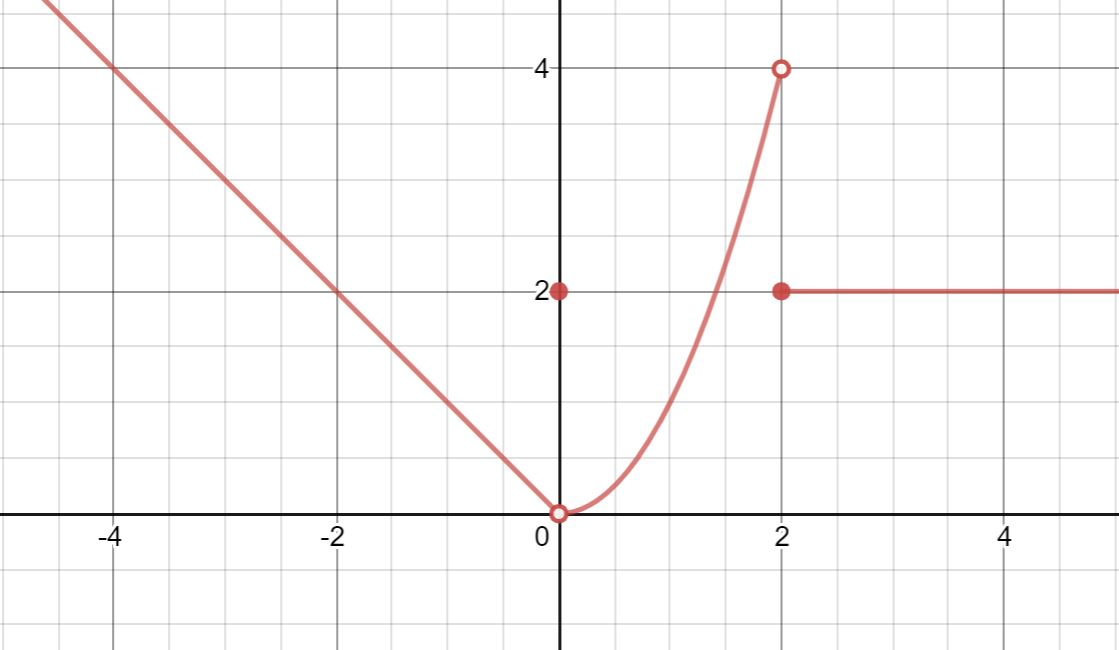
\includegraphics[height=1in]{240finalimage1.jpg}

\end{image}

$$\lim_{x\rightarrow 0^-}f(x)=\answer{0},\,\lim_{x\rightarrow 0^+}f(x)=\answer{0},\,\lim_{x\rightarrow 0}f(x)=\answer{0}$$
$$\lim_{x\rightarrow 2^-}f(x)=\answer{4},\,\lim_{x\rightarrow 2^+}f(x)=\answer{2},\,\lim_{x\rightarrow 2}f(x)=\answer{dne}$$

  \end{enumerate}
\end{problem}

\begin{problem}\label{prob:mth240finalprob2}
State the limit definition of the derivative.
$$f'(x)=\lim_{h\rightarrow 0}\frac{\answer{f(x+h)}-\answer{f(x)}}{\answer{h}}$$
\end{problem}

\begin{problem}\label{prob:mth240finalprob3}
For each of the following find $\frac{dy}{dx}$.
  \begin{enumerate}
\item
$$y=\sin (x^2+1)$$
$$\frac{dy}{dx}=\answer{2x\cos(x^2+1)}$$

\item
$$y=x^7(x^2-3)^8$$
$$\frac{dy}{dx}=\answer{7x^6(x^2-3)^8}+\answer{16x^8(x^2-3)^7}$$

\item
$$xy=\cos y$$
$$\frac{dy}{dx}=\answer{\frac{-y}{x+\sin y}}$$
  \end{enumerate}
\end{problem}

\begin{problem}\label{prob:mth240finalprob4}
Find the equation of the tangent line to the graph of $y=\frac{1}{x}$ at $x=2$.

Show your steps:
$$\frac{dy}{dx}=\answer{-x^{-2}}$$
$$\frac{dy}{dx}\Big|_{x=2}=\answer{\frac{-1}{4}}$$
$$\mbox{slope of the tangent line: }m=\answer{\frac{-1}{4}}$$
$$\mbox{point on the line: }(2, \answer{0.5})$$
$$\mbox{equation of the tangent line: }y=\answer{-0.25x+1}$$
\end{problem}

\begin{problem}\label{prob:mth240finalprob5}
A hot air balloon is rising vertically at a rate of 1 meter per second.  An observer is standing 90 meters away from the point directly underneath the balloon.  How fast is the distance between the observer and the balloon increasing when the balloon is 100 m above the ground.

\begin{image}
   
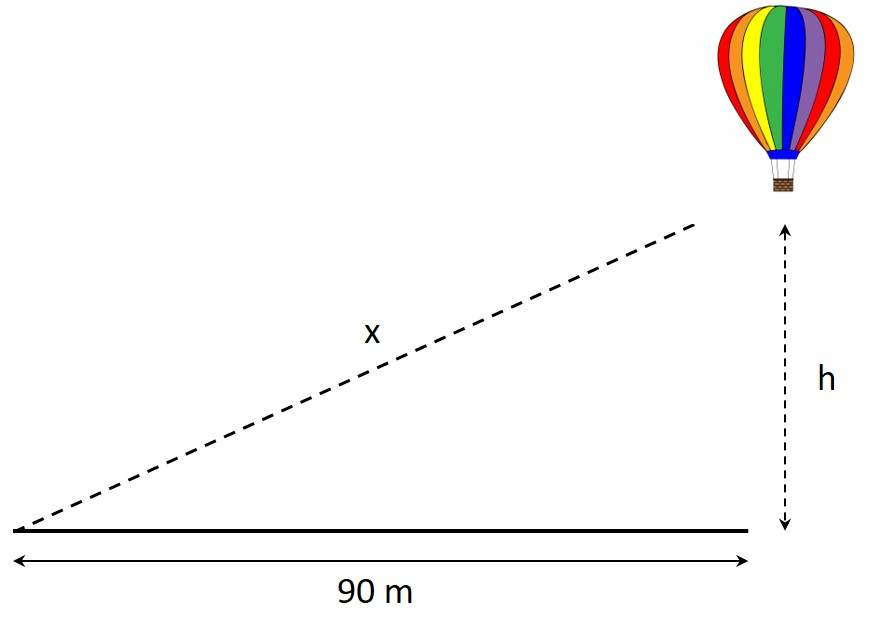
\includegraphics[height=1in]{240finalimage2.jpg}

\end{image}

Given rate: $\frac{dh}{dt}=\answer{1}$.

Find rate:  $\frac{dx}{dt}$

Relationship between $\answer{h}$ and $\answer{x}$:

$$\answer{h^2}+90^2=\answer{x^2}$$

When $h=100$, $x=\answer[tolerance=0.1]{134.5}$.

When the balloon is 100 m above the ground, the distance between the observer and the balloon is changing at the rate of $\answer[tolerance=0.01]{0.74}$ meters per second.
\end{problem}

\begin{problem}\label{prob:mth240finalprob6}
Integrate.
  \begin{enumerate}
\item
$$\int (\sqrt{x}+x)dx=\answer{\frac{2}{3}x^{\frac{3}{2}}+0.5x^2}+C$$

\item
$$\int \frac{1}{x^2}dx=\answer{-x^{-1}}+C$$
\end{enumerate}
\end{problem}

\begin{problem}\label{prob:mth240finalprob7}
Evaluate the definite integral 
  
$$\int_{-1}^{1} (x^2-2x)dx=\answer{\frac{2}{3}}$$
\end{problem}

\begin{problem}\label{prob:mth240finalprob8}
The graph of $f(x)=-3x^2+2x+4$ is shown below.  Find the area of the shaded region.
\begin{image}
   
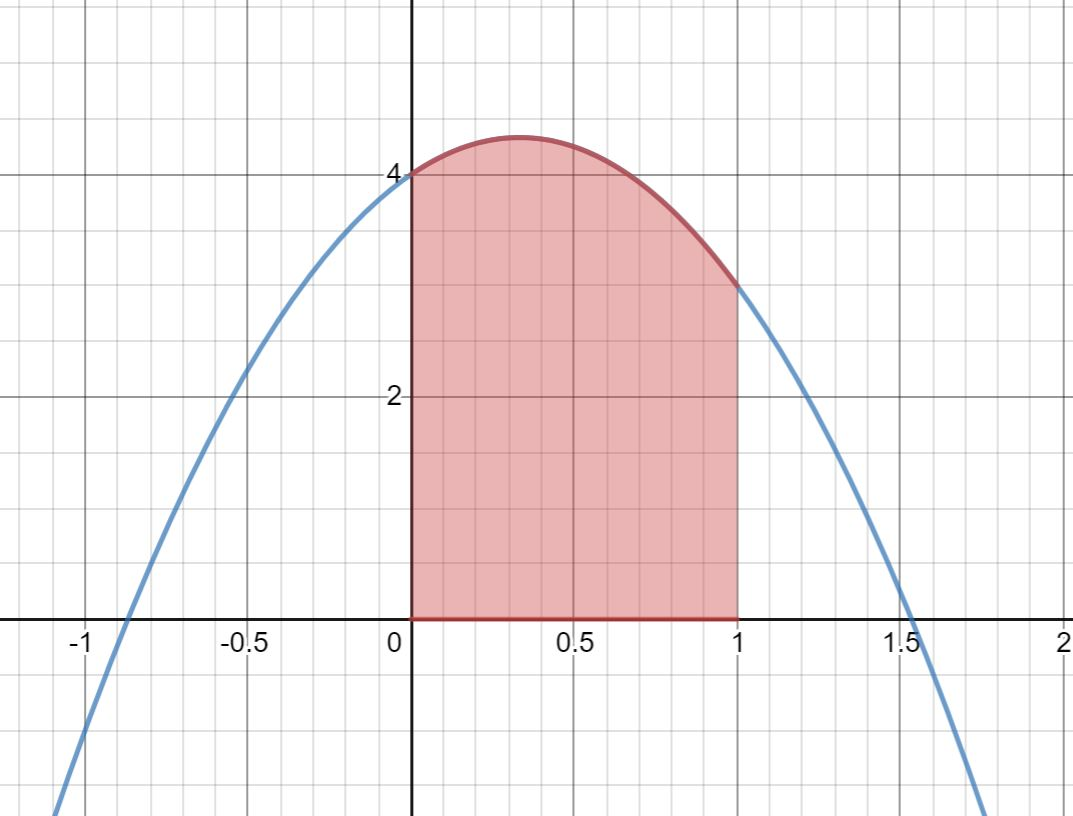
\includegraphics[height=1in]{240finalimage3.jpg}

\end{image}
Area of the shaded region:
$$\int_{\answer{0}}^{\answer{1}}\answer{-3x^2+2x+4}\,dx=\answer{-x^3+x^2+4x}\Big|_{\answer{0}}^{\answer{1}}=\answer{4}$$
\end{problem}

\begin{problem}\label{prob:mth240finalprob9}
Let $f(x)=\frac{1}{3}x^3+300x^2+9x$.  Find the intervals on which the function $f$ is concave up and concave down.

The function is concave down on 
$$\Big( \answer{-\infty}, \answer{-300}\Big)$$
The function is concave up on
$$\Big( \answer{-300}, \answer{\infty}\Big)$$

\end{problem}


\end{document} 